\begin{document}
Nach der Analyse von verschiedenen Visualisierungsmethodiken musste der Umfang und die Komplexität der Applikation bestimmt werden.
Folgende Kriterien wurden festgelegt:
\begin{itemize}
    \item Visualisierung sollte unspezifisch auf Daten funktionieren
    \item Benutzer sollte in der Lage sein, die Struktur des Grafen selbst zu bestimmen
    \item 3D Welt sollte ohne weitere Benutzer Interaktion generiert werden
\end{itemize}
Des weiteren wurde festgelegt, das die Webseite mit dem Framework ''ReactJS'', das zeichnen und erstellen der 3D Welt wird anhand des Framework
''AFrame'' realisiert und der Server der die Webseite veröffentlicht wird soll mit ''NodeJS'' geschrieben werden. \\
Die Applikation wird anhand des Package Managers ''npm'' aufgesetzt.

\section{Installieren, Transpilieren des Client \& Starten des Server}
Da die Applikation über den PackageManager npm verwaltet und aufgesetzt wird, ist die Applikation namentlich in zwei Ordner unterteilt.
\begin{itemize}
    \item Server
    \item Client
\end{itemize}
Diese beinhalten je eine tsconfig.json und package.json und im falle des Client eine webpack.config.js.
\begin{itemize}
    \item package.json \\ \\
        Die package.json beinhaltet alle Abhängigkeiten des Clients oder Servers. Man muss diese über den Befehl ''npm install''
        für jede Instanz installieren.
    \newpage
    \item webpack.config.js \\ \\
        Die webpack.config.js beschreibt ''webpack'' wie das Projekt aufgesetzt ist und welche Gegebenheiten beim Transpilieren bedacht werden
        müssen. ''Webpack'' ist ein Modul welches mehrere JavaScript Dateien, in eine große JavaScript Datei bündelt. Der Zweck hiervon ist das man
        diese Einfach in einem Browser einbinden kann. \\
        Um einen Prozess zu haben der Konsequent die Dateien überwacht (develop server), muss man den Befehl ''npm start-watch'' Ausführen.
        Dieser startet intern zwei Prozesse die Asynchrone laufen. Der Prozess ''webpack --watch'' welches die Typescript Dateien in
        JavaScript transpiliert und der Befehl ''node-sass --watch ...'' welches die Stylesheets kompiliert. \\
        Um für einen Release zu bauen reicht der Befehl, ''npm run start-build'' aus.
    \item tsconfig.json \\ \\
        Die tsconfig.json beschreibt dem TSServer der die Typescript Dateien überwacht, nach welchen Standards sie geschrieben werden
        müssen.
\end{itemize}
\newpage

\section{Server}
Die Entscheidung einen Server zu schreiben hat mehrere Gründe auf die ich in diesem Kapitel kurz eingehen werde. \\ \\
Einer der Gründe ist das die Anwendung über einen Server veröffentlicht werden muss um diesen auf einen herkömmlichen Server im Internet
hochladen zu können. Der Server kann aus dem namentlichen Ordner mit dem Befehl, ''npm run prod'' gestartet werden.  Man bedenke das vorher
der Client mindestens einmal über den befehlt ''npm run start-build'' transpiliert werden muss, oder ein laufender build Server über den
Befehl ''npm start'' existieren sollte. Der Server holt daraufhin die Dateien vom Client und über die Adresses "localhost:6080" im Browser
erreichbar.\\ \\
Ein weiterer Grund war, das in dem Design Prozess die Idee existierte, einen MongoDB Server über eine Docker Instanz
zu verwalten. Dieser würde die Datenstruktur, die Ausgewählt und Generiert wurde, abspeichern und zur abfrage jederzeit bereit halten. \\ \\
Wie sich später auch herausstelle wäre der finale Grund den Server zu verwenden, dass Browser einen lokalen Cache Limit haben. Somit können
größere Dateien (500 MB und größer) nicht mehr direkt vom Browser verarbeitet werden. Diese müssten in einer produktiv Umgebung erstmal auf
den Server hochgeladen. Dort analysiert, verarbeitet und umgewandelt werden, und zu guter Letzt wieder zu der Anwendung zurück geschickt
werden. \\
\newpage

\section{Applikation}
Basierend auf den Kriterien wurde die Funktionalität der Anwendung in drei Abschnitte unterteilt.
\begin{itemize}
    \item Anzeige \& Konfiguration
    \item Analyse
    \item Welt Generierung
\end{itemize}
Zu dem musste ich mir in diesem Stadium schon Gedanken machen wie meine Daten in der Praxis aussehen würden also wurde Datenquellen wie
IMDB angeschaut. IMDB gibt seine Daten im TSV Format raus. Somit wurden die Formate CSV, TSV oder JSON als Formate definiert die, die
Applikation verarbeiten können muss. Mit diesem Wissen ging ich an die Logik ran diese Daten anzuzeigen und zu konfigurieren.

\subsection{Anzeige \& Konfiguration}
Die Anzeige \& Konfiguration der Daten wird wiederum über drei Schritte absolviert. Zuerst muss eine valide csv, tsv oder json (json in einer
flachen Hierarchie) ausgewählt werden.
\begin{lstlisting}
                                Beispiel JSON
[
    {
        id: "0",
        title: "Geschichte des VR",
        author: "Walter Guenther",
        veroeffentlicht: "1996"
    },
    {
        id: "1",
        title: "Datenvisualisierung 101",
        author: "Peter Watson",
        veroeffentlicht: "2001"
    }
]
\end{lstlisting}
\newpage \noindent
Falls eine CSV oder TSV Datei ausgewählt wurde, wird dieser intern verarbeitet und anhand eines D3 Moduls umgewandelt. Ein teil des Inhaltes wird
dem Benutzer veranschaulicht. In folgendem Beispiel verwenden wir den ein teil des Datensatzes von IMDB und zeigen dem Benutzer die ersten 10 Einträge mit allen
vorhandenen Attributen und ihren zugehörigen Werten an.
\begin{center}
    
\includegraphics[width=0.75\textwidth]{File-Selection.png}
    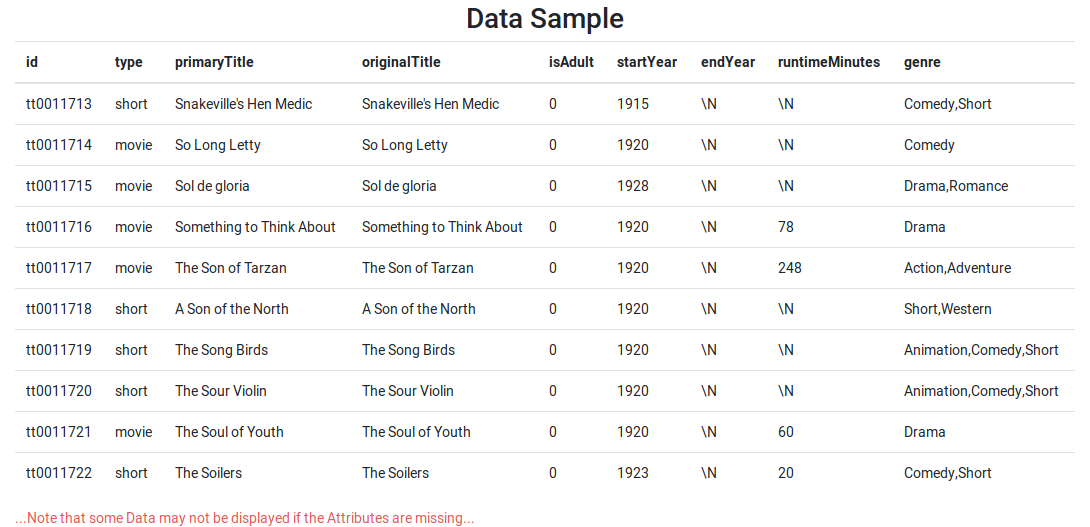
\includegraphics[width=0.75\textwidth]{File-Content.png} \\
\end{center}
Hiernach wird dem Benutzer die Option angeboten, ein primären und sekundären Parameter auszuwählen. Des weiteren können weitere Werte definiert
werden die im sekundären Knoten visualisiert werden.
\begin{center}
    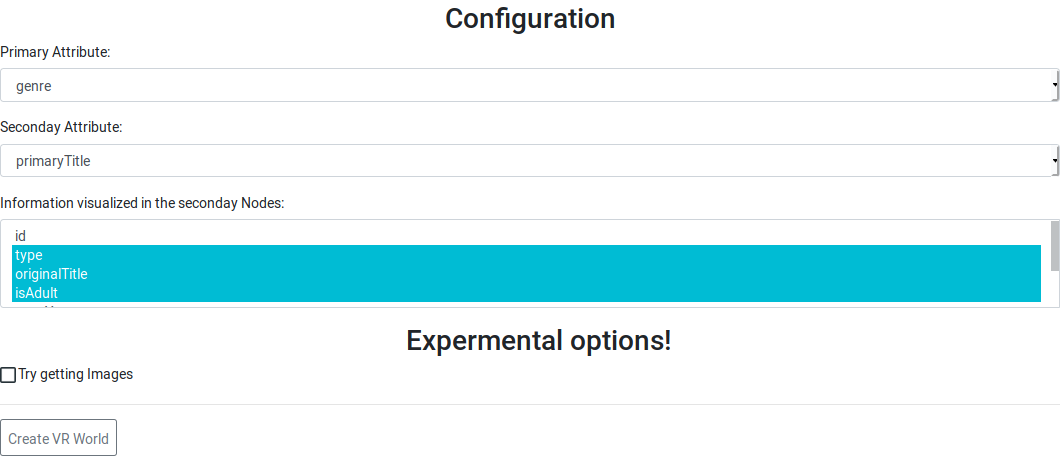
\includegraphics[width=0.75\textwidth]{Configuration-Part.png} \\
\end{center}
Die Idee anhand des sekundär Wertes Bilder zu finden wurde in Erwägung gezogen jedoch nach genauerem nachdenken wegen der Spezialisierung
auf dem IMDB Datensatz verworden. Diese ausgewählten Attribute werden verwendet und eine Parent, Child Hierarchie zu erstellen. 
Wenn man nur die oben ersehbaren Daten in Betracht zieht. Wird nach der Auswahl von den Attributen, eine interne Datenstruktur generiert
die visuell Dargestellt wie Folgt aussieht.
\begin{center}
    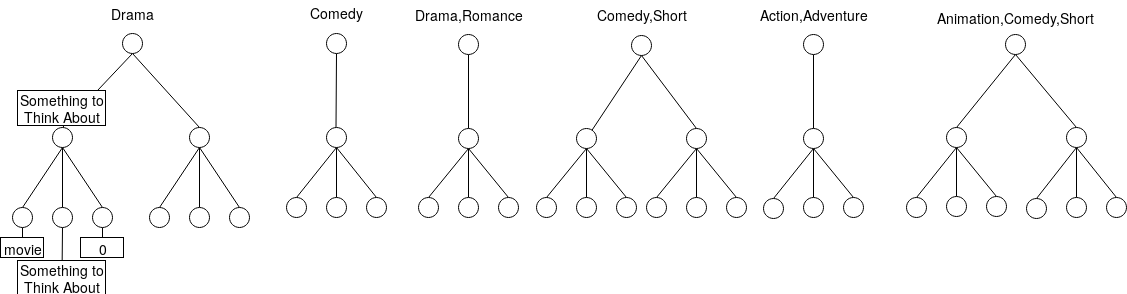
\includegraphics[width=1\textwidth]{Internal-Datastructure.png}\label{setup_data} \\
\end{center}

\newpage
\subsection{Visualisierung der Daten}
Mit dem Klick auf ''Create VR World'' werden die Daten an eine Scene weitergeleitet, womit anhand des Frameworks A-Frame eine 3D Welt
generiert wird. Bei der Generierung dieser Welt mussten Probleme wie übersicht der Daten und größe der Welt beachtet werden. \\
Wenn die Datensätze sehr groß sind, wird die Welt dementsprechend groß. Um dieses zu vermeiden wird der Datensatz vor der Generierung
in kleine Portionen von 30 Objekten unterteilt. Heißt wenn der Datensatz 200 Objekte beinhaltet wird dieses in sieben Unterszenen verteilt.
Durch diesen Schritt wird die Performanz der Anwendung gesteigert und die übersicht der Daten verbessert. \\
Eine zirkuläre Verteilung der Haupt- und Unterknoten wird in diesem Projekt als die Hauptmethode der Visualisierung verwendet. Um hierfür
eine sinnvolle Verteilung der Daten zu erreichen, wird dynamisch für jeden Hauptknoten, ein Position in einem Radius abhängig von der größe
der Sektion ermittelt.
\begin{center}
    \begin{equation*}
        position=
        \begin{bmatrix}
            radius * Math.cos((index / length) * 2 * Math.PI) \\
            y \\
            radius * Math.sin((index / length) * 2 * Math.PI)
        \end{bmatrix}
    \end{equation*}
\end{center}
Dies führt dazu das die Knoten, egal wie viele, gleichmäßig in einem Kreis verteilt sind. Die selbe Formel wird zur Berechnung der
positionen der Unterknoten verwendet, jedoch werden diese relative zur Wurzel verschoben. \\
Bei den Unterknoten werden, um die Übersicht zu steigern, ebenfalls Untergruppen erzeugt und auf der y-Achse gestapelt. Gleichzeitig werden
diese zuerst versteckt gezeichnet und müssen über die Interaktion mit dem Hauptknoten eingeblendet werden.
\begin{center}
    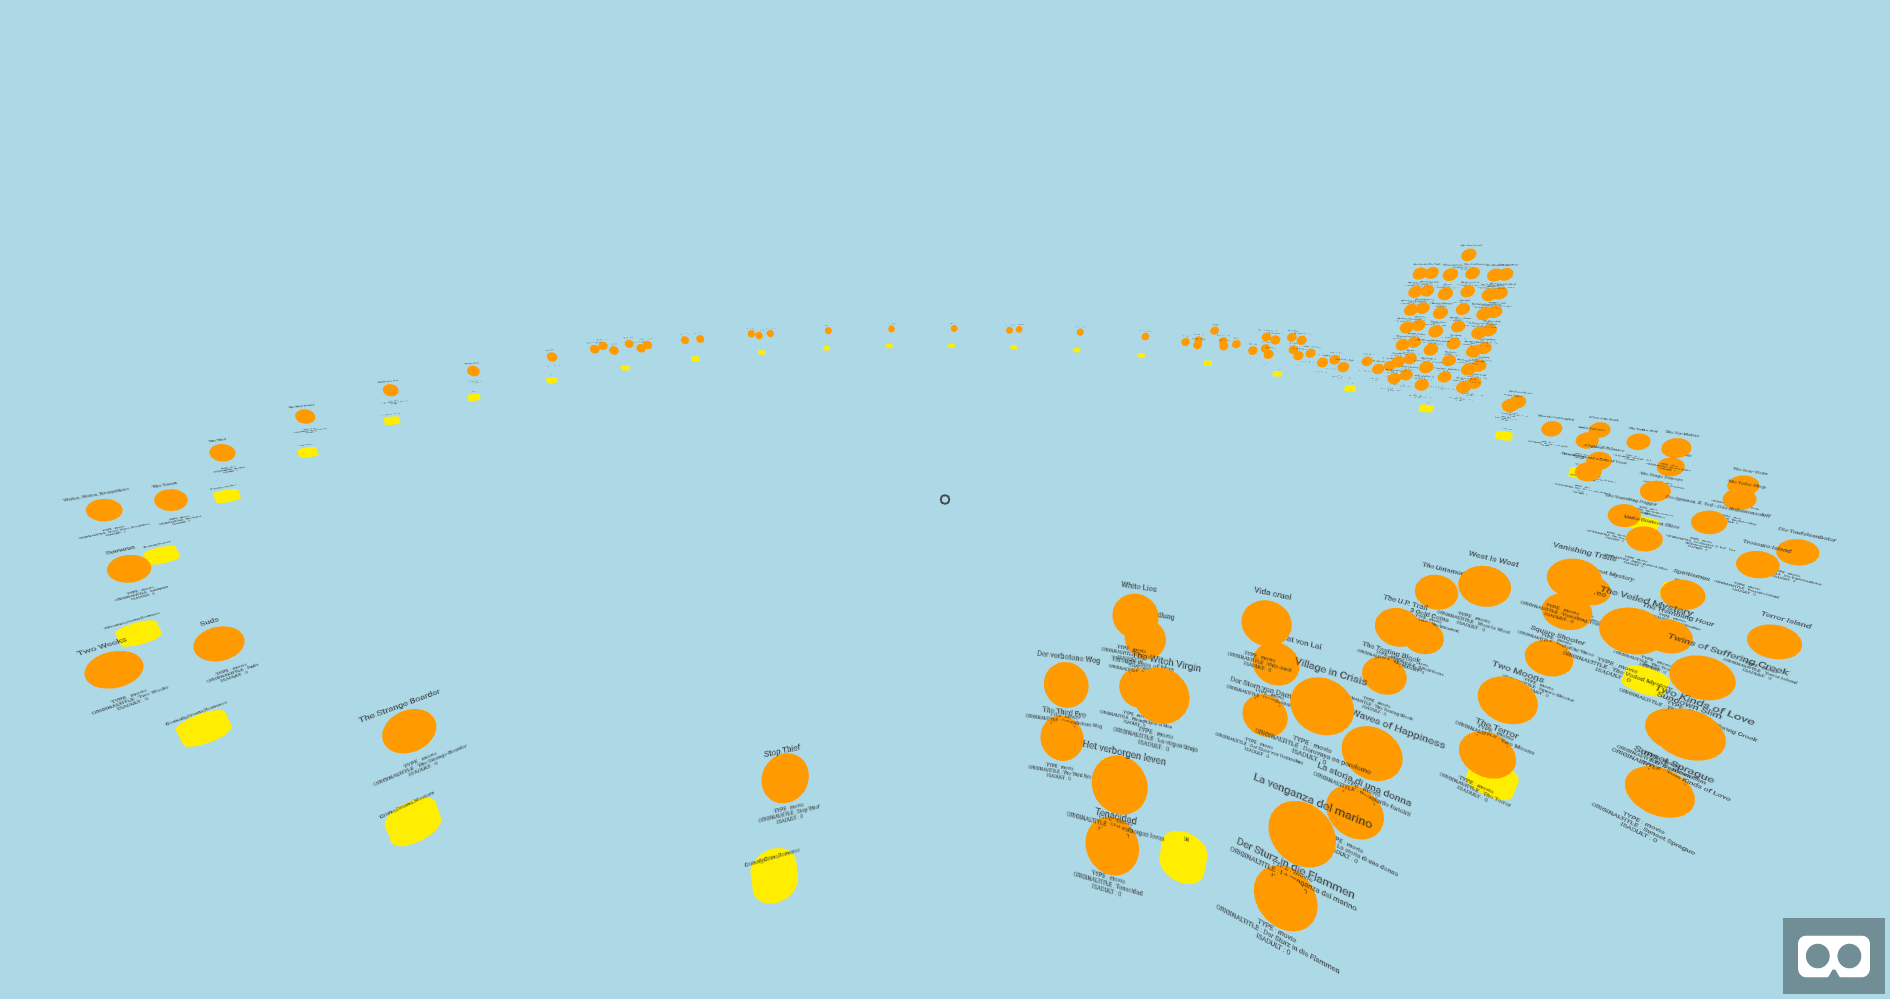
\includegraphics[width=1\textwidth]{3D-visualization.png}
\end{center}

\newpage
\subsection{Interaktionen in der Applikation}
Für die Interaktion in der Applikation wurden eigene Events definiert und geschrieben.\\\\
Um unterknoten Einzublenden, muss auf den Hauptknoten mit der Mausgeklickt oder per Controller X(Playstation), A(XBox) gedrückt werden.\\\\
Die Kamera im VR und Normal Modus kann per Controller oder Tastatur (wasd) gesteuert werden. Die Steuerung per Controller geschieht wie gewohnt
mit dem linken Joystick. Die Höhe der Kamera wird mit der vorderen rechten und linken Schultertaste gesteuert.\\\\
Das wechseln von Scenen / Sektionen geschieht über das Drücken des linken und rechten Analog tasten, links fürs nächstes- und rechts für
vorherige Scene.
\end{document}
